\begin{figure}[H]
\begin{center}
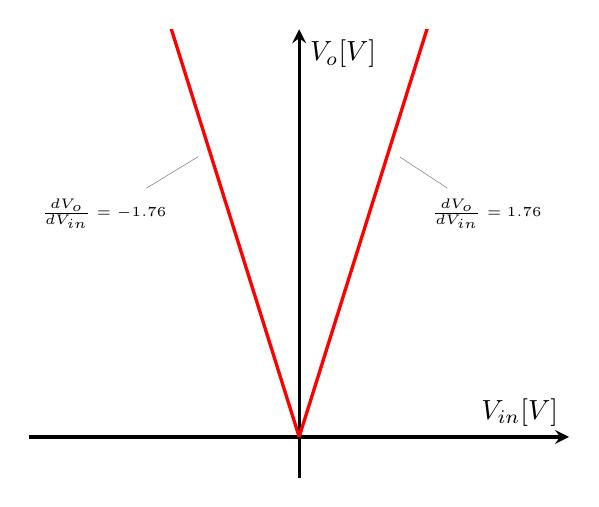
\begin{tikzpicture} 
\begin{axis}[very thick,
                     samples = 100,
                     ytick={-10,10},
                     xlabel = {$V_{in}[V]$},
                     ylabel = {$V_{o}[V]$},
                     xmin = -6,
                     xmax = 6,
                     ymin = -0.5,
                     ymax = 5,
                     axis x line = middle,
                     axis y line = middle,
                     ticks = none]
            \addplot[draw=red, domain=-4:0] plot (\x, {-1.76*\x});
            \addplot[draw=red, domain=0:4] plot (\x, {1.76*\x});
            \addplot[mark=none] coordinates {(-2,3.52)} node[pin=230:{\tiny $\frac{dV_o}{dV_{in}}=-1.76$}]{};
            \addplot[mark=none] coordinates {(2,3.52)} node[pin=-50:{\tiny $\frac{dV_o}{dV_{in}}=1.76$}]{};
        \end{axis}
\end{tikzpicture}
\end{center}
\caption{Característica de transferência para o retificador de onda completa de precisão.}
\label{graph:2} 
\end{figure}